\section{The ribosome as a missing link in prebiotic evolution II: Ribosomes encode ribosomal proteins that bind to common regions of their own mRNAs and rRNAs}

\subsection{Нормальное название}

Рибосома как недостающее звено в эволюции пребиотиков II: рибосомы кодируют рибосомные белки, которые связываются с общими участками их собственных мРНК и рРНК.

\subsection{Абстракт}
Авторы предположили, что рибосома может представлять собой недостающее звено между пребиотической химией и первыми клетками. Одно из предположений, которое следует из этой гипотезы, которую мы здесь проверяем, заключается в том, что рибосомная РНК(рРНК) должна кодировать белки, необходимые для функционирования рибосом. Другими словами, рРНК также функционировала пребиотически как мРНК. Поскольку эти связывающие рибосомы белки (rb-белки) должны связываться с рРНК, но рРНК также функционирует как мРНК, отсюда следует, что rb-белки также должны связываться со своей собственной мРНК. Эту гипотезу можно противопоставить «нулевой» гипотезе, согласно которой rb-белки возникли независимо от последовательностей рРНК, и поэтому не должно быть необходимого сходства между рРНК, с которой связываются rb-белки, и мРНК, кодирующей rb-белок.

\subsubsection{Пояснения к вышеуказанному}
Они представляют 5 доказательств своей теории: 1) повсеместное связывание rb-белков с их собственными мРНК и аутогенный контроль их собственной трансляции, 2) более высокая, чем ожидалось, частота появления богатых аргинином модулей, связанных со связыванием РНК, которое происходит в белках, кодируемых рРНК, 3) факт, что рРНК-связывающие области rb-белков гомологичны своим мРНК-связывающим областям, 4) более высокая, чем ожидалось, встречаемость последовательностей rb-белка, кодируемых в рРНК, которые имеют высокую степень гомологии с их мРНК, по сравнению со случайным выбором других белков, 5) рРНК у современных прокариот и эукариот кодирует функциональные белки.


Ну и еще они предлагаются дальнейшие проверки гипотезы: (1) экспериментальное тестирование того, связываются ли белки, кодируемые рРНК, с рРНК в их кодирующих сайтах; (2) кодируются ли тРНК-синтетазы, которые, как известно, связываются со своими собственными мРНК, самими последовательностями тРНК; (3) и предсказание того, что геномы архей и прокариот (основанные на ДНК) были построены вокруг «генов» рРНК, так что последовательности, связанные с рРНК, будут составлять неожиданно высокую долю этих геномов.

\subsection{Картинки}
\begin{figure}[H]\label{ul}
	\center{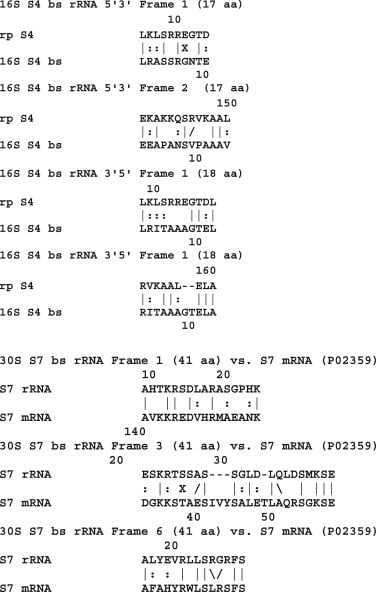
\includegraphics[scale=0.7]{a11.jpg}}
	\caption{Первая картинка}
\end{figure} 
Тут они сравнивают последовательности рибосомальных белков на мРНК и рРНК. Сплошная линия - совпадает, пунктир - комплементарные, а крестик - не знаю).
\begin{figure}[H]\label{ul}
	\center{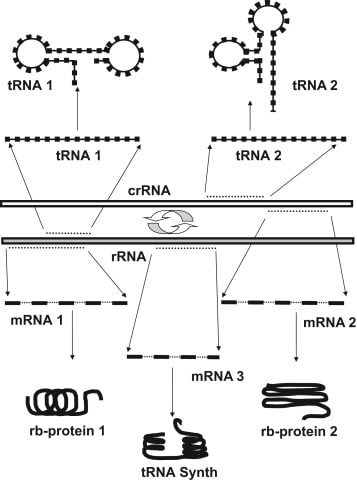
\includegraphics[scale=0.7]{a12.jpg}}
	\caption{Вторая картинка}
\end{figure} 
Здесь нарисованы основные функции кодирования информации в этой теории. По центру - рРНК, может кодировать и мРНК и тРНК + может транскрибировать в комплементрную последовательность, которая также будет кодировать мРНК и тРНК.
\begin{figure}[H]\label{ul}
	\center{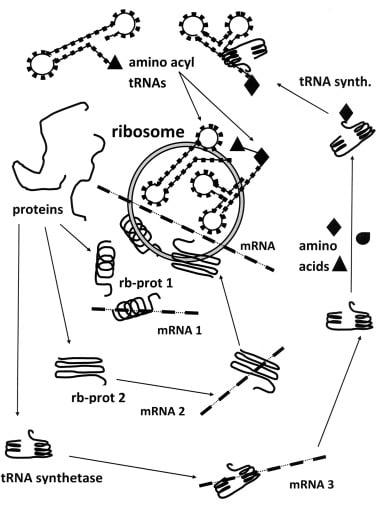
\includegraphics[scale=0.7]{a13.jpg}}
	\caption{Третья картинка}
\end{figure} 
Здесь нарисовано, как компоненты второго рисунка взимодействуют с целью создания функционирующей рибосомы, способной осуществлять трансляцию и просто метаболический контроль. рРНК (жирный серый кружок в центре)связывает рибосомальные белки. Эти rb-белки не только обеспечивают рибосомные функции, такие как помощь в связывании тРНК, но также автогенно регулируют свое собственное производство путем связывания с последовательностями мРНК, гомологичными их сайтам связывания рРНК. Некоторые из этих белков также выполняют дополнительные метаболические функции, такие как присоединение аминокислот к соответствующим тРНК для создания аминоацил-тРНК, которые используются рибосомой для синтеза пептидов или белков. Результатом этого является саморегулируемая система управляемой рибосомой репликации, транскрипции и трансляции, которая кодирует все компоненты, необходимые для репликации рибосомы.